\chapter{基于全局表示的局部特征提取在神经文本分类中的应用}

\section{引言}
在文本分类任务中,有一种非常主流的方法。该方法首先利用显式的局部抽取器来识别关键的局部特征,然后再根据这个识别好的特征进行分类,我们将这一研究领域称为``局部特征驱动模型''。

\begin{table}[t]
  \begin{center}
    \begin{tabular}{c c}
    \toprule
    % Case1: \emph{\textbf{Apple} is amazing extremely in taking photos.}\\
    示例1: \emph{\textbf{苹果}太棒了! 我已经受够了我的相机了。}\\
	% Case2: ``\emph{People store \textbf{apples} in root cellar during the winter for their own use or for sale.}"\\
	% Case2: ``\emph{All fifteen of the Bayfield \textbf{Apple} Company products are made at our orchard.}"\\
	示例2: \emph{\textbf{苹果}享誉世界,并且值得被称为 ``营养宝仓''.}\\
    \bottomrule
    \end{tabular}
  \end{center}
  \caption{主题分类中的\emph{科技}和\emph{健康}, \emph{\textbf{``苹果''}} 的意思在局部文本中难以被正确的区分。}
\label{tab: case}
\end{table}

许多方法都可以归入这个范围。在传统机器学习中,ngram是一种非常有用的方法~\citep{pang2002humbs, wang2012baselines}。而对于深层神经网络,将局部特征编码成低维的分布式向量,用ngram嵌入,并对其进行简单的组合,取得了很不错的效果~\citep{joulin2016bag, qiao2018anew}。
卷积神经网络(CNN)~\citep{lecun2010convolutional},由于具有很强的捕获局部特征平移不变性的能力,在文本分类中受大学者的广泛应用。
最近,~\citecf{wang2018disconnected}提出了分解递归神经网络(Disconnected Recurrent Neural Network, DRNN),它利用RNN来提取更大窗口的局部特征,并在几个基准数据集上取得了最好的结果。

尽管目前基于局部特征提取方法虽然具有良好的可解释性和不错的性能,但仍然存在一个缺点。
如表\ref{tab: case}所示,``苹果''可能指的是一种水果,也可能指的是一个科技公司。而由于他的歧义,我们只能从句子的整体意境才能正确地识别出``苹果''的真正含义。如果负责``苹果''的局部特征提取器从一开始无法接收到``相机''和``营养'',我们便需要更加复杂的上层结构来帮助修改不够精确的局部表示``苹果'',从而创建新的高级特征用于最后的分类。
一般,我们可以通过深度堆叠\citep{Jords201201Dead,conneau2016very}和混合集成\citep{xiao2016efficient}进行高价特征的组合。
不过这种复杂的堆叠模型,训练效率低,难度大,尤其是在语料库不足的情况下。

为了解决这个问题,我们认为一个更有效的方法是直接优化局部提取过程,在此想法上,本文提出了一种新的体系结构Encoder1-Encoder2。
之前的工作通常只使用一个编码器,而我们的结构中包含了两个编码器,分别用于相同的输入序列。
具体来说,Encoder1可以是任何一种神经网络模型,它的作用是简单掌握该句的全局背景知识。而Encoder2是一个局部特征驱动模型。我们将Encoder1生成的全局表示加入到Encoder2的局部特征提取过程中。这样,局部特征提取器(Encoder2)就可以注意到更多的全局背景知识。因此,由于对全局背景信息的感知,Encoder2可以更好地捕捉特定并与该实例相关的局部特征。我们直接用Encoder2的结果进行分类,这也意味着我们可以避免其他的复杂操作。

我们在公开的8个分类数据集上进行了实验,实验结果表明我们提出的结构可以明显地提高局部特征驱动模型。在不使用任何无监督方法的情况下,我们的模型在所有基准数据集上取得了最佳效果。此外,我们也进一步证明了我们的模型在半监督领域的泛化性。


\section{Encoder1-Encoder2结构}
\begin{figure*}[ht]
\center
     % \includegraphics[width=0.85\textwidth]{model2.pdf}
     \includegraphics[width=0.85\textwidth,height=6.5cm]{model2.pdf}
     %\caption{Encoder1-Encoder2 Architecture. Encoder1 servers as a global information provider while Encoder2 is a local feature driven model whose output is directly fed into the classifier. S and A indicate two Interaction Modes between Encoder1 and Encoder2. }
     \caption{Encoder1-Encoder2结构由三部分组成。 (1) Encoder1是全局信息提供器。 (2) Encoder2是局部特征抽取器,它的结果直接用于分类。(3) Mode是二者的交互模式,其中``S''和``A''分别是``SAME''模式 and ``ATTEND''模式的缩写。}
     \label{fig:models}
\end{figure*}

\subsection{整体介绍}

本文提出了一种新的文本分类神经网络结构Encoder1-Encoder2,如图\ref{fig:models}所示。相同的输入序列将被两个编码器分别编码两次,但只有编码器2的输出直接用于分类器。具体地说,Encoder1是提供全局信息的先锋,而Encoder2通过将前者合并到局部提取过程中来集中于提取更好的局部特征。此外,为了更具针对性地吸收全球信息,还发展了两种交互模式。

\subsection{Encoder1: 全局信息提供器}
在不丧失通用性的情况下,我们在我们的架构中引入了三种类型的Encoder1模型,每种模型都可以是独立的全局信息提供者,并在我们的实验中进行了比较。

\textbf{CNN模型: } 假设$\mathbf{x}_t$是表示长度为${n}$的句子的第$t$个词的$d$维词向量, $\mathbf{x}_{t-h+1:t}$ 代表宽度为$h$的词的组合$\mathbf{x}_{t-h+1}, \mathbf{x}_{t-h+2}, \ldots, \mathbf{x}_{t}$。我们使用$k$个核对输入的句子进行特征提取。
正式地,核$\mathbf{W}_f$作用于窗口$\mathbf{x}_{t-h+1:t}$得到$\mathbf{h}_{t}$。
\begin{align}
% \begin{equation}
% \begin{split}
\mathbf{h}_{t} &= Conv(\mathbf{x}_{t-h+1}, \mathbf{x}_{t-h+2}, \ldots, \mathbf{x}_{t}) \label{equ: conv}\\
			   &= relu(\mathbf{W}_f \mathbf{x}_{t-h+1:t} + \mathbf{b}_f)
% \mathbf{enc_1} = [\mathbf{c}_{1}, \mathbf{c}_{2}, \ldots; \mathbf{c}_{n}]
% \end{split}
% \end{equation}
\end{align}

通过相同补齐的方式,我们对$n$个窗口进行特征提取,则全局信息可以被表示为$\mathbf{enc}_1$:

\begin{equation}
\mathbf{enc}_1 = [\mathbf{h}_{1}; \mathbf{h}_{2}; \ldots; \mathbf{h}_{n}]
\end{equation}

\textbf{GRU模型: } Gated recurrent units (GRU,门控循环神经网络)是将门控机制引入RNN的一种网络结构~\citep{cho2014learning}。
GRU中使用两种类型的门:重置门决定更新多少新信息,而更新门控制以前信息的流。
隐藏状态$\mathbf{h}_{t}$是基于$\mathbf{h}_{t-1}$和$\mathbf{x}_{t}$迭代计算的。
% \begin{equation}
% \mathbf{h}_{t} = GRU(\mathbf{x}_{1}, \mathbf{x}_{2}, \ldots, \mathbf{x}_{t})
% \end{equation}

\begin{gather}
\label{equ: gru1}
\mathbf{r}_{t} = \sigma(\mathbf{W}_{r} \mathbf{x}_{t} + \mathbf{U}_{r} \mathbf{x}_{t-1} + \mathbf{b}_{r}) \\
\mathbf{z}_{t} = \sigma(\mathbf{W}_{z} \mathbf{x}_{t} + \mathbf{U}_{z} \mathbf{x}_{t-1} + \mathbf{b}_{z}) \\
\hat{\mathbf{h}_{t}} = \tanh(\mathbf{W}_{h} \mathbf{x}_{t} + \mathbf{U}_{h} (\mathbf{r}_{t} \odot \mathbf{x}_{t-1}) + \mathbf{b}_{h}) \\
\mathbf{h}_{t} = (1 - \mathbf{z}_{t}) \odot \mathbf{h}_{t-1} + \mathbf{z}_{t} \odot \hat{\mathbf{h}_{t}}
\label{equ: gru2}
\end{gather}

因此,可以对所有先前的信息进行编码。我们将其缩写为:
\begin{equation}
\mathbf{h}_{t} = GRU(\mathbf{x}_{1}, \mathbf{x}_{2}, \ldots, \mathbf{x}_{t})
\end{equation}

全局信息是所有时刻的隐状态,即:
\begin{equation}
\mathbf{enc}_1 = [\mathbf{h}_{1}; \mathbf{h}_{2}; \ldots; \mathbf{h}_{n}]
\end{equation}

\textbf{注意力机制: }
此外,像\citecf{zhou2016attention}一样,我们还在GRU上引入了注意机制,以提高对有价值信息的关注度。
定义上下文向量$\mathbf{u}_{w}$以衡量GRU中每个隐藏状态$\mathbf{h}_{t}$的重要性,该值是随机初始化的并会在训练过程中不断学习。
我们采用了softmax函数以得到归一化的重要性权重$\alpha_{t}$:

\begin{equation}
{\alpha_{t}} = \frac{\exp({\tanh(\mathbf{h}_{t})}^\top \mathbf{u}_{w})} {\sum_{t} \exp({\tanh(\mathbf{h}_{t})}^\top \mathbf{u}_{w})}
\end{equation}
通过注意力机制得到的全局信息表示如下:
\begin{equation}
\mathbf{enc}_1 = [\alpha_{1}\mathbf{h}_{1}; \alpha_{2}\mathbf{h}_{2}; \ldots; \alpha_{n}\mathbf{h}_{n}]
\end{equation}

\subsection{Encoder2: 新颖的局部特征提取器}
\label{encoder2}
之前我们提到的局部特征抽取器都被严格限定在有限大小的区域,这里我们提出了一种新颖的方法。除了预期的局部上下文外,由Encoder1提取的全局信息也被局部特征提取器吸收。这样,由Encoder2提取的局部特征可以注意到全局背景信息,并仍然保持的局部信息的平移不变性。
对于Encoder2,我们介绍了两种局部特征驱动模型,即CNN和DRNN。
假设$\mathbf{g_t}$是某一个确定大小的窗口中所需的全局信息,我们将会在\ref{interact}中详细介绍它。

\textbf{CNN模型: } 这里我们将 $\mathbf{g_t} \in \mathbb{R}^{d}$ 当作全局信息,并且使其和窗口中的单词一起做卷积。基于公式 \ref{equ: conv}, 从窗口$\mathbf{x}_{t-h+1:t}$中提取的局部信息可以表示为:
\begin{equation}
\mathbf{h}_{t} = Conv(\mathbf{g_t}, \mathbf{x}_{t-h+1}, \mathbf{x}_{t-h+2}, \ldots, \mathbf{x}_{t})
\end{equation}

\textbf{DRNN模型:}
与CNN不同,DRNN利用RNN为每个窗口提取局部特征~\citep{wang2018disconnected}。为了将全局信息引入DRNN,伪造的全局信息$\mathbf{g_t}$会像CNN一样填充在每个窗口的头部。由于RNN的序列性,即使是在有限的窗口中,全局信息也可以从头开始编码到RNN中,并对后面的词产生影响。这里我们使用GRU作为局部特征提取模型,窗口$\mathbf{x}_{t-h+1:t}$产生的特征可以表示为:

\begin{equation}
\mathbf{h}_{t} = GRU(\mathbf{g_t}, \mathbf{x}_{t-h+1}, \mathbf{x}_{t-h+2}, \ldots, \mathbf{x}_{t})
\end{equation}

为了维持平移不变性,我们在CNN和DRNN模型之后都采用了最大池化操作,池化的结果便是Encoder2的输出:
\begin{equation}
\mathbf{enc}_2 = maxpool([\mathbf{h}_{1}; \mathbf{h}_{2}; \ldots; \mathbf{h}_{n}])
\end{equation}


\subsection{Encoder1和Encoder2间的交互模式}
\label{interact}

假设Encoder1提供的全局信息为$\mathbf{enc}_1$,特定窗口宽度为$h$的局部输入$\mathbf{x}_{t-h+1:t}$需要的全局信息为$\mathbf{g_t}$,其中$G$是交互模式的函数:

\begin{equation}
\mathbf{g_t} = G(\mathbf{enc}_1, \mathbf{x}_{t-h+1}, \mathbf{x}_{t-h+2}, \ldots, \mathbf{x}_{t})
\end{equation}

从两种不同的想法出发,我们提供了两种交互模式。

\textbf{SAME模式:}我们把$\mathbf{enc}_1$当作一个由Encoder1提供的``参考书"。在SAME模式里,无论该窗口本身的局部信息如何,每一个窗口都会得到来自全局信息相同的指导。因此,我们在$\mathbf{enc}_1$之后接入一个最大池化层,以此来提取最有价值的参考信息。
\begin{equation}
\hat{\mathbf{g_t}} = maxpool(\mathbf{enc}_1)
\end{equation}

\textbf{ATTEND模式}:
ATTEND模式从另一个角度来利用全局信息。根据该窗口不同的上下文,Encoder1的指导信息可以更有针对性。具体来说,我们使用注意力机制来获取Encoder1中不同的参考信息。

对于宽度为$h$的窗口$\mathbf{x}_{t:t+h-1}$,我们将该窗口中所有的词求和,得到该窗口的向量表示,则Encoder1中每一个隐层的重要性权重$\alpha_{t}$ 可以通过下式来计算:

\begin{equation}
{\alpha_{t}} = \frac{\exp({\tanh(\mathbf{h}_{t})}^\top avg(\mathbf{x}_{t:t+h-1}))} {\sum_{t} \exp({\tanh(\mathbf{h}_{t})}^\top avg(\mathbf{x}_{t:t+h-1}))}
\end{equation}

为了最大化的使用Encoder1中的所有信息,我们将最大池化和注意力机制得到的结果连接起来,则ATTEND模式中最后得到的参考信息为:
\begin{equation}
\hat{\mathbf{g_t}} = Concat(maxpool(\mathbf{enc}_1), \sum_{t} \alpha_t \mathbf{h}_{t})
\end{equation}

为了和单词的输入向量保持一致,我们使用全连接层将$\hat{\mathbf{g_t}}$压缩到 $\mathbf{g_t}$。这样,这个全局信息向量可以很容易地被嵌入到Encoder2的局部特征提取过程。

\subsection{分类层}
在将从Encoder1获得的全局信息合并到Encoder2的局部特征提取过程中之后,后者的输出向量可以看作是整个文本的表示。然后我们将该向量输入softmax分类器以预测每个类别的概率,并使用交叉熵作为损失函数,其中$\hat{y}_{i}$是预测的概率,而$y_i$是类$i$的真实概率:
\begin{gather}
\hat{y} = softmax(\mathbf{W}_{c}\mathbf{enc}_2  + \mathbf{b}_c)\\
%{y} = softmax(\mathbf{W}_{c}\mathbf{X}  + \mathbf{b}_c)\\
{H(y,\hat{y})} = \sum_{i}{y}_{i}\log\hat{{y}_{i}}
\end{gather}


\section{实验}
我们进行了实验以验证模型的效果,并和之前的方法进行对比。

\subsection{数据集}

我们采用了公开数据集验证我们的模型\cite{zhang2015character}。
这些数据集包含不同的领域,包括情感分析、新闻分类、问答分类和本体分类,我们在表\ref{tab:datasets}中进行了总结。

\begin{table}[t]
  % \small  
  % \begin{small}
  \begin{center}
  % \scalebox{0.8}{
    \begin{tabular}{lccccc}
    \toprule
      Dataset & 类别 & 句子长度 & 数据集大小 & 测试集 & 任务 \\
      \midrule
      Yelp P. & 2 & 156 & 560k & 38k & 情感分类 \\
      Yelp F. & 5 & 158 & 650k & 50k & 情感分类  \\
      Amz. P. & 2 & 91 & 3M & 650k & 情感分类 \\
      Amz. F & 5 & 93 & 3.6M & 400k & 情感分类 \\
      AG & 4 & 44 & 120k & 7.6k & 新闻分类\\
      Sogou & 5 & 579 & 450k & 60k & 新闻分类\\
      Yah. A. & 10 & 112 & 1.4M & 60k & 问题分类\\
      DBP & 14 & 55 & 560k & 70k & 本体分类\\
    \bottomrule
    \end{tabular}
  % }
  \end{center}
\caption{数据集概述}
\label{tab:datasets}
% \end{small}
\end{table}

\subsection{模型设置}

在数据预处理方面,我们使用NLTK提供的预处理包对所有的文本进行分割、词性还原等操作\citep{loper2002nltk}。
模型超参方面,所有的符号都和\ref{encoder1}以及\ref{encoder2}保持一致。
对Encoder1,我们采用了CNN,GRU和Attention。
在CNN中(Encoder1),我们用了窗口大小为$[3,5,7]$的窗口,每一个窗口有128个不同的卷积核。
GRU (Encoder1) 和 Attention (Encoder1)的隐层大小都是128。

对于Encoder2,我们分别在CNN和DRNN这两种局部特征抽取模型中进行实验。
在CNN(Encoder2)中,有窗口大小分别为$[3,5,7]$的卷积核,每种窗口都有128个。
在DRNN(Encoder2)中,所有的隐层大小为300。
其他的模型设置在表\ref{tab: settings}中,包括词向量在内的所有训练参数都是随机初始化的,没有使用任何预训练的手段\citep{mikolov2013distributed,peters2018deep,devlin2018bert}。
\begin{table}[t]  % [h]表格在文中放置的位置
  \centering  %作用是使表格居中
  \small
  \begin{center}
    \begin{tabular}{lccc}
    \toprule
    语料 & 词表大小 & 句子长度 & 窗口大小 \\ 
    \midrule
      Yelp P. & 150k & 300 & 20  \\
      Yelp F. & 200k & 300 & 20  \\
      Amz. P. & 400k & 256 & 15  \\
      Amz .F. & 400k & 256 & 15  \\
      AG & 50k & 128 & 15  \\
      Sogou & 56k & 400 & 15  \\
      Yah. A. & 400k & 256 & 20  \\
      DBP & 400k & 128 & 15  \\
    \bottomrule
    \end{tabular}
  \end{center}
\caption{模型设置,我们限定了词汇表大小并设置了最大句长。此外,我们按照\citecf{wang2018disconnected}设定了DRNN模型中的窗口大小。}
\label{tab: settings} %表格标签 方便引用
\end{table}

\subsection{训练及评估}
对于每个数据集,我们将整个训练语料随机分成训练和验证集,其中验证集大小与相应的测试集大小相同。
之后我们将验证集固定,以便进行公平比较。
我们用验证集误差最小的模型,进行测试,并汇报了测试结果。

我们选择了AdaDelta \cite{zeiler2012adadelta}($\rho=0.95$ ,$\epsilon=1e-6$)作为优化器,并使用了梯度裁剪以防止梯度爆炸的问题。
我们在所有包含了RNN结构的模型中加入了L2正则化。在Yelp P. 和Yelp F. 数据集中,批处理大小为64,在其他数据集中,批处理大小都被设置为128。
我们采用了早停技术,早停值为10。

\begin{table*}[ht]
% \begin{small}
  \begin{center}
  \scalebox{0.9}{
    \begin{tabular}{lcccccccc}
      \toprule
      模型 & Yelp P. & Yelp F. & Amz. P. & Amz. F. & AG & Sogou & Yah. A. & DBP \\
      \midrule
      bigram-FastText \citep{joulin2016bag}   & 95.7 & 63.9 & 94.6 & 60.2 & 92.5 & 96.8 & 72.3 & 98.6 \\
      Region-emb \citep{qiao2018anew}   & 96.2 & 64.5 & 95.3 & 60.8 & 92.8 & \underline{97.3} & 73.4 & \underline{98.9} \\
      \midrule
      SANet(big) \citep{letarte2018importance}   & 95.2 & 64.0 & 95.5 & 61.3 & 92.6 & -    & 74.1 & 98.8 \\
      \midrule
      LSTM  \citep{zhang2015character}    & 94.7 & 58.2 &  93.9 & 59.4  &  86.1  & 95.2 & 70.8 & 98.6 \\
      D-LSTM  \citep{yogatama2017generative}    & 92.6 & 59.6 & -    & -    & 92.1 & 94.9 & 73.7 & 98.7 \\

      \midrule
      char-CNN \citep{zhang2015character}  & 94.7 & 62.0 & 94.5 & 59.6 & 87.2 & 95.1 & 71.2 & 98.3 \\
      % char-CRNN \citep{cho2014learning}    & 94.5 & 61.8 & 94.1 & 59.2 & 91.4 & 95.2 & 71.7 & 98.6 \\
      VDCNN \citep{conneau2016very}     & 95.7 & 64.7 & \underline{95.7} & \underline{63.0} & 91.3 & 96.8 & 73.4 & 98.7 \\
      \midrule
      \midrule

      CNN \citep{kim2014convolutional}    & 95.8 & 64.7 & 95.2 & 60.9 & 91.9 & 97.1 & 72.6 & 98.8 \\
      \emph{Encoder1}-CNN-S (Ours)     & 96.5 & 66.2 & 95.9 & \textbf{63.3} &  92.5  & \textbf{97.5} & 74.5 & 98.8 \\
      \emph{Encoder1}-CNN-A (Ours)   & 96.5 & 66.5 & \textbf{96.0} & \textbf{63.3} &  93.0  & \textbf{97.5} & 74.6 & 98.9 \\
      \midrule

      DRNN  \citep{wang2018disconnected}      & \underline{96.3} & \underline{66.4} & {95.6} & \underline{63.0} & \underline{92.9} & 96.9 & \underline{74.3} & \underline{98.9} \\
      \emph{Encoder1}-DRNN-S (Ours)    & 96.6 & 66.8 & \textbf{96.0} & 63.2 & 93.0 & 97.2 & 74.8 & \textbf{99.0} \\
      \emph{Encoder1}-DRNN-A (Ours)      & \textbf{96.7} & \textbf{67.0}  & \textbf{96.0} & 63.1 & \textbf{93.2}  & 97.3 & \textbf{75.0} & \textbf{99.0} \\
     \bottomrule
    \end{tabular}
    }
  \end{center}
    \caption{各数据集中测试集准确率[\%]。
    % Baseline models are CNN \citep{kim2014convolutional} and DRNN \citep{wang2018disconnected}, which are chosen as encoder2 in our architecture.
    我们使用Encoder1-Encoder2-Mode来代表我们的结构,其中``S''代表``SAME''而``A''代表``ATTEND''模式。
    % We only list the best performance of specific Encoder2 in SAME and ATTEND mode respectively. 
    % For example, we report the best results in row Encoder1-CNN-S where Encoder2 is CNN \citep{kim2014convolutional} and Interaction Mode is SAME with different Encoder1.
    对于某一种Encoder2,我们测试了三种不同的Encoder1。
    % For the sake of brevity, we only list the best performance here.
    为了简介, \emph{Encoder1}这里代表了这三种不同的Encoder1模型中最佳的结果,而不是某一种Encoder1。
    % We list the best performance of three Encoder1 for specific Encoder2 and Interaction Mode.
    % Detailed experiments results for all combinations of Encoder1-Encoder2-Mode are reported in supplementary materials. 
    至于用来对比的模型, 第一块列举了基于n-grams的模型,包括bigram-FastText \citep{joulin2016bag}和region embedding \citep{qiao2018anew}. 自注意力网络SANet \citep{letarte2018importance}放在第二块中.
    基于RNN的模型LSTM \citep{zhang2015character}, D-LSTM  \citep{yogatama2017generative}和基于CNN的模型char-CNN \citep{zhang2015character} 和VDCNN \citep{conneau2016very}列在第三和第四块中。 强力的局部特征提取模型CNN \citep{kim2014convolutional} 和DRNN \citep{wang2018disconnected} 作为基线模型被列在最后两块,且被拿来直接和我们的模型对比。}
  \label{tab:results}
% \end{small}
\end{table*}
\subsection{实验结果和分析}
表\ref{tab:results}展示了实验结果。我们使用下划线来代表最好的公开模型,并用粗体表明最好的结果。在我们提出的架构中,我们最好的模型在所有8个文本分类基准数据中上都超过了以前的最佳模型。

在公开模型中,几乎所有的最佳结果都是由局部特征驱动模型(包括region emb、VDCNN和DRNN)取得的。
自注意力模型SANet表现良好,但并没有取得像在seq2seq(序列到序列)场景中那样好的效果,基于RNN的方法也没有。
我们认为,这是因为关键短语和词序在文本分类中起着更关键的重要作用。



\begin{figure*}[ht]
    \centering
    \begin{subfigure}[]{0.45\textwidth}
        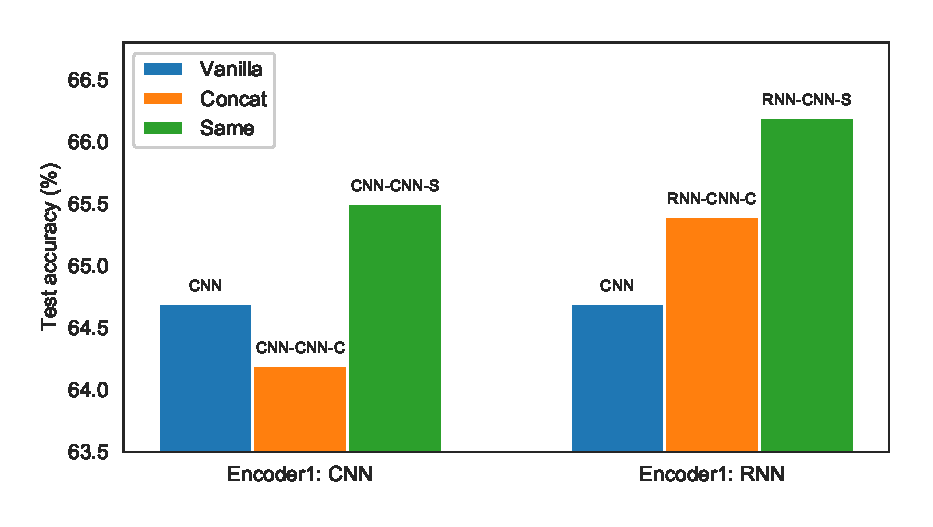
\includegraphics[width=\linewidth]{S-C1.eps}
        \caption{Experiments on Yelp F.}
        \label{fig:S1}
    \end{subfigure}
    ~
    \begin{subfigure}[]{0.45\textwidth}
        \includegraphics[width=\linewidth]{S-C2.eps}
        \caption{Experiments on Yah. A.}
        \label{fig:S2}
    \end{subfigure}
    \caption{模型拆解实验。 ``Vanilla''是最传统的CNN模型 \citep{kim2014convolutional}. ``Concat''只concat(连接)Encoder1和Encoder2的输出,并根据连接的结果直接分类。 ``Same'' 代表了我们框架中的交互模式。}
    \label{fig: Ablation}
\end{figure*}

对于我们的模型,实验结果表明,使用全局编码器的增强局部抽取器在性能上优于普通的局部抽取模型。当选择CNN作为局部特征提取器时,模型对于一些相对困难的任务提升尤为显著,例如Amz. F.(+2.4\%) 和Yah. A.(+2.0\%)。

Encoder1-CNN比具有29个卷积层的VDCNN性能更好。考虑到我们的局部抽取器是非常简单的CNN,是只有一层的浅层模型,这个结果是很不错的。此外,复杂的VDCNN在大型数据集如Amz. P.(95.7\%)和Amz. F.(63.0\%)中表现最好,但在较小的数据集如AG(91.3\%)表现一般。而我们的Encoder1-CNN在所有数据集上都有很好的效果。
当DRNN作为局部特征抽取器时,我们加入的全局编码器提高不像CNN中那么大,但仍然相当稳定。Encoder1-DRNN在所有数据集上都优于DRNN,最高值可以可达到0.7\%。
